\documentclass[11pt]{article}
\usepackage[ansinew]{inputenc}
%\usepackage[utf8]{inputenc}
\usepackage[numbers]{natbib}
\usepackage{hyperref}
\usepackage[pdftex]{color,graphicx,epsfig}
\DeclareGraphicsRule{.pdftex}{pdf}{.pdftex}{}
\usepackage{amssymb,amsmath}
\usepackage{multirow}
\usepackage{hyperref}
\usepackage{lscape}
\usepackage{longtable}
\usepackage{color}
\usepackage{fancyvrb}
\usepackage{enumerate}
\usepackage{float}
\usepackage{setspace}
\usepackage{natbib}





\newcommand{\Rlogo}{\protect\includegraphics[height=1.8ex,keepaspectratio]{./figures/Rlogo.pdf}}
\newenvironment{itemize*}%
  {\begin{itemize}%
    \setlength{\itemsep}{-0.35cm}%
    \setlength{\parskip}{10pt}}%
  {\end{itemize}}
\usepackage[pdftex]{graphicx}
\usepackage{tikz} 
\usetikzlibrary{shapes,arrows} 
\usepackage[a4paper,left=2cm,right=2cm,top=1.5cm,bottom=1.5cm]{geometry}



\newenvironment{changemargin1}{
  \begin{list}{}{
    \setlength{\leftmargin}{+5cm}
    \setlength{\rightmargin}{3cm}
    \footnotesize
  }
  \item[]
  }{\end{list}}



\begin{document}


\title{\Large \bf {{\tt compareGroups} Web User Interface (WUI) Tutorial}}


\vspace{0.5cm}


\author{Isaac Subirana$^{1,2,3}$}

\maketitle

\begin{scriptsize}
\noindent $^{1}$CIBER Epidemiology and Public Health (CIBERESP), Spain \\
$^{2}$IMIM - Parc de Salut Mar, Barcelona \\
$^{3}$Statistics Department, University of Barcelona, Spain \\
\end{scriptsize} 


\begin{center}
\texttt{isubirana@imim.es}
\end{center}

\vspace{0.5cm}

\tableofcontents


\vspace{2cm}

%%%%%%%%%%%%%%%%%%%%%%%%%%%%%%%%%%%%%%%%%%%%%%%%%%%%%%%%%%%%%%%%%%%
\section{Introduction} \label{section-Introduction}

The {\tt compareGropus} package (version $\geq$ 2.1) incorporates a Web User Interface (WUI) based on {\tt shiny} {\tt R} package \citep{Shiny} (\href{http://shiny.rstudio.com}{http://shiny.rstudio.com}) to use all functionality of the package very easily and quickly for non {\tt R} users.\\

This application includes almost all the options existing in `type on' version. Also, thanks to the power of {\tt shiny} package, the user can see the results when setting the included variable, the groups, number of decimals, etc almost instantaneously (`reactivity' -see {\tt shiny} manual and examples-). This is very useful to modify and customize the descriptive table before saving it in the desired format saving a lot of time.\\

In the following sections, we list and describe all the options available in the {\tt Shiny}- {\tt compareGroups} application, and we illustrate how it works with a real example.




%%%%%%%%%%%%%%%%%%%%%%%%%%%%%%%%%%%%%%%%%%%%%%%%%%%%%%%%%%%%%%%%%%%
\section{Menus and options} \label{section-menus}

Once the WUI is called, a web browser is launched with two main parts: in the left hand side there are all the control menu options to read the data frame from different format files, select the variables list to be analysed, specify the number of digits of the descriptives or p-values displayed in the bivariate table, and much more other aspects; while the right hand side contains the results, i.e, a table containing a basic summary of all variables, the bivariate table or some plots.\\

Following, an exhaustive list describing all the options are presented:


%%%%%%%%%%%%%%%%%%%%%%%%%%%%%
\subsection{Control menu (left side)}

\begin{itemize}

\item \color{blue} START \color{black} 
   A panel with all the options to select the data base and to select the analysed variables. Different file formats are allowed; in the present version these are: SPSS, plain text (txt or csv), EXCEL (2000 or 2007) or {\tt R} (.rda or RData). Also, it is possible to select example data already present in the {\tt compareGroups} package (REGICOR and PREDIMED) and SNPS from {\tt SNPassoc} package.

\item \color{blue} SETTINGS \color{black}    
   A panel with different issues to control for different aspects of the bivariate table:

	\begin{itemize}
	\item \color{blue} Type \color{black} Each variable can be analysed as normal or non-normal or as categorical. In the first case, mean and standard deviation are displayed; for the second case, medians and quantiles; and for the latest, frequencies and proportions.
	\item \color{blue} Response \color{black} Control menu to select which variable indicates the group. Three choices are possible:
		\begin{enumerate}[1)]
		\item {\bf None:} descriptives are performed for the entire data set with no groups.
		\item {\bf Group:} a variable must be selected. By default, only factor variables with five or less categories can be selected. The descriptives will be performed by these groups. When the grouping variable has only 2 categories, Odds Ratio (OR) can be computed.
		\item {\bf Survival:} to perform survival analysis where the response is a right censored variable,i.e., with time variable and a variable indicating the censoring (i.e., whether or not the individual suffered the disease). Also, the disease or case status must be indicated.
		\end{enumerate}
	\item \color{blue} Hide \color{black} For categorical variables, select the category you want to be hidden. Additionally, in the `hide no' input text windows you can type the category which represents `no' in the sense that the category named as indicated for all binary variables are hidden.
	\item \color{blue} Subset \color{black} A global subset can be typed affecting all analysed variables. Also you can select a subgroup of individuals for each variable. In any case, a logical expression in {\tt R} language must be typed:
   		\begin{center}
		\begin{tabular}{cc}
		\hline
		Operator & {\tt R} \\
		\hline
		= & == \\
		or & | \\
		and & \& \\
		not & ! \\
		\hline
		\end{tabular}
		\end{center}
Note that to indicate the category, you must type the number that appears in the `VALUES' table on right side of the application instead of its name. For example, for gender, type 1 instead of `male' and 2 instead of `female', if `male' is the first category and `female' is the second.
	\item \color{blue} OR/HR \color{black} Options for Odds Ratio (OR) when response is binary or Hazard Ratios (HR) for right censored response. You can specify the reference category when computing the OR or HR for the categorical variables. For continuous variables, the scale can be changed. This is very useful for variables with a wide range such as total cholesterol, where it makes more sense to display the OR/HR for each 10 units of change rather than a single unit.
	\end{itemize}
\item \color{blue} DISPLAY \color{black} 
  In this panel, the user can select which information must be displayed in the resulting bivariate table, and in which format, etc.
	\begin{itemize}
	\item \color{blue} Show \color{black} What to be displayed in the bivariate table:
		\begin{itemize}
		\item {\bf ALL:} Descriptives for the entire data set.
		\item {\bf p-overall:} p-value comparing the means, medians, proportions or incidence among groups.
		\item {\bf Descriptives:} Descriptives (means, medians, proportions, etc.) by groups.
		\item {\bf p-trend:} p-value for trend. It is supposed that the groups are ordered.
		\item {\bf OR/HR:} Odds Ratio or Hazard Ratio for binary or time-to-event response (grouping variable), respectively.
		\item {\bf Available:} Number of individuals with valid data for each variable and each groups.
		\item {\bf NA category:} For categorical variables, the non-available data is considered as a new category.
		\item {\bf Pairwise p-value:} When more than two groups are considered, p-values corresponding to 2 by 2 comparisons are performed taking into account multiple testing.
		\item {\bf Simplify:} Empty categories (with no available data) are removed from the analyses.
		\end{itemize}
	\item \color{blue} Format \color{black} The user can specify how to display the mean and standard deviation, the quantiles
and frequencies.
	\item \color{blue} Decimals \color{black} The number of decimals to be displayed in the bivariate table, for descriptives, p-values and for OR / HR.
	\item \color{blue} Labels \color{black} This tab allows to change the `key' headers of the descriptive table such as `ALL', `p-value', etc.
	\end{itemize}	
\item \color{blue} SAVE \color{black}
  A panel with the options to save both the bivariate table or the plots. Depending on the active results tab (right side), i.e., tables or plots, different options are displayed.
\end{itemize}



%%%%%%%%%%%%%%%%%%%%%%%%%%%%%%%%%
\subsection{Results panels (right side)}

\begin{itemize}

\item \color{blue} INFO \color{black}
  A table showing the available data for each variable and possibly each group, as well as some other information such as the selection criteria, etc.

\item \color{blue} VALUES \color{black}
  Using this tab, the user can take a look at the data contained in the data set.

  \begin{itemize}
  \item \textbf{Summary:} A table with the the name, label and a basic summary of all the variables contained in the data set.
  \item \textbf{Extended:} A table with the raw values in the data set. By default only the first ten rows are displayed, but the user can set the number of rows to be shown and navigate through the data set.
  \end{itemize}

\item \color{blue} TABLE \color{black} 
  The bivariate table. It can be displayed in three different formats: HTML, PDF or as
it is printed in the {\tt R} console. Note that, although this is the less nice format, it is the fastest option to be displayed and, in consequence, may be the most useful way to see how the bivariate table looks like when some options are modified (e.g. grouping variable) `on line'.

\item \color{blue} PLOT \color{black} 
  Univariate or bivariate (taking into account the groups if proceeds) plots of selected
variable.

\item \color{blue} SNPs \color{black} 
  Descriptives of SNPs (Single Nucleotide Polymorphims) with appropriate statistics and
tests for these genetic variants. To perform this analysis, only SNPs variables can be selected. A factor response to display genotype frequencies by groups is permitted but not a time-to-event response variable.

\item \color{blue} HELP \color{black} 
  Use this tab to know more about {\tt compareGroups} and its Web User Interface.
  \begin{itemize}
  \item \textbf{About:} Explanation about both the {\tt compareGroups} R-package and its Web User Interface (WUI) version. Also, it contains the security rules of the data sent by the user when using WUI remotely (from {\tt www.comparegroups.eu}). 
  \item \textbf{Panel:} Help navigation panel that mimics both the control and result panels.
  \end{itemize}

\end{itemize}




\newpage
%%%%%%%%%%%%%%%%%%%%%%%%%%%%%%%%%%%%%%%%%%%%%%%%%%%%%%%%%%
\section{Example}


In this section we illustrate how to analyse a data set.


\begin{itemize}

\item {\bf Step 0. Launch the WUI application on a web browser}. To use the WUI locally (and not on a remote server), first load the {\tt compareGroups} package and call the {\tt cGroupsWUI} function:
\color{blue}
\begin{verbatim}
> library(compareGroups)
> cGroupsWUI()
\end{verbatim}
\color{black}

\item {\bf Step 1. Load the data and select the variables to be analysed}
In this example we will load the PREDIMED data set from the PREDIMED study \citep{PREDIMED}. This data is already available in the {\tt compareGroups} package. 
We will select all variables except the event and the time-to-event variable (`toevent'). They will represent the response and must be removed from the row-variables.
\begin{center}
\fbox{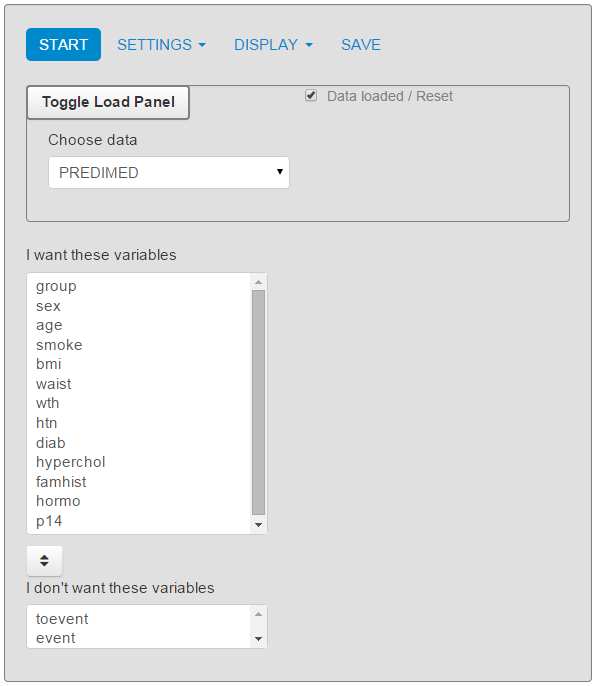
\includegraphics[width=0.6\textwidth]{./figures/WUI/step1.png}}
\end{center}

\vspace{0.5cm}

\newpage
\item {\bf Step 2. Select the grouping variable.}
Since PREDIMED is a longitudinal study where the main goal is to check whether the mediterranean diet is related to a less incidence of cardiovascular disease, we will take the response as the time to cardiovascular event. To do so, we will select `Survival' response type, setting the `toevent' as time variable and `event' as indicator variable (taking `yes' as case).
\begin{center}
\fbox{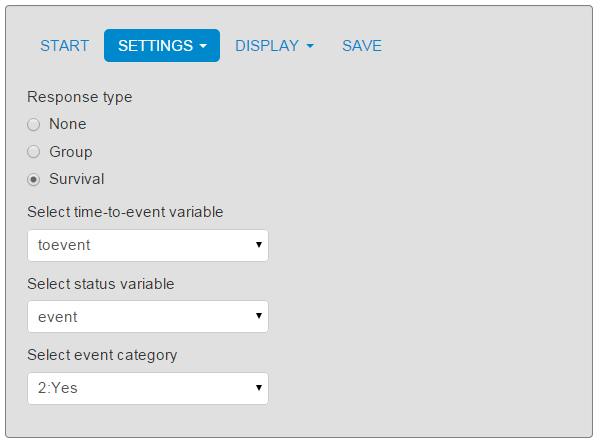
\includegraphics[width=0.55\textwidth]{./figures/WUI/step2.png}}
\end{center}

\vspace{0.5cm}
\item {\bf Step 3. Take a look at the plots} to see which continuous variables should be treated as normal and which not. By default, {\tt compareGroups} performs a Shapiro-Wilks normality test to decide which variables are normal. But we may want to check the normality assumption graphically.
\begin{center}
\fbox{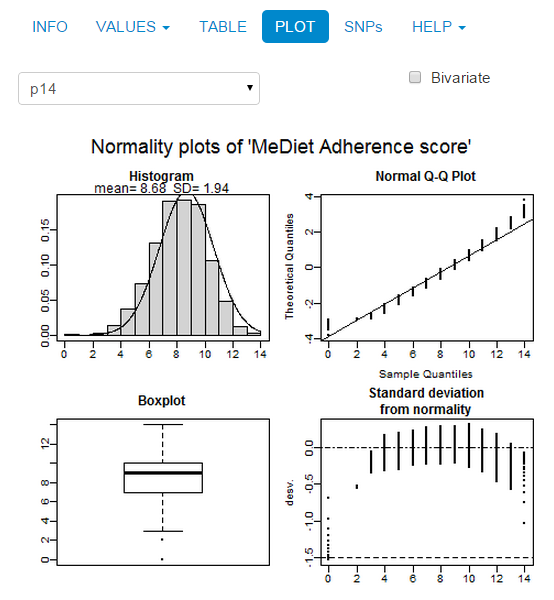
\includegraphics[width=0.55\textwidth]{./figures/WUI/step3.png}}
\end{center}

\newpage
\item {\bf Step 4. Set the options.}

	\begin{itemize}
	
	\item {\bf Type:} Specify the variables to be treated as normal and the ones as non normal. To specify that all of them will be treated as normal, except `p14' for which median and quartiles are displayed instead of mean and SD:
\begin{center}
\fbox{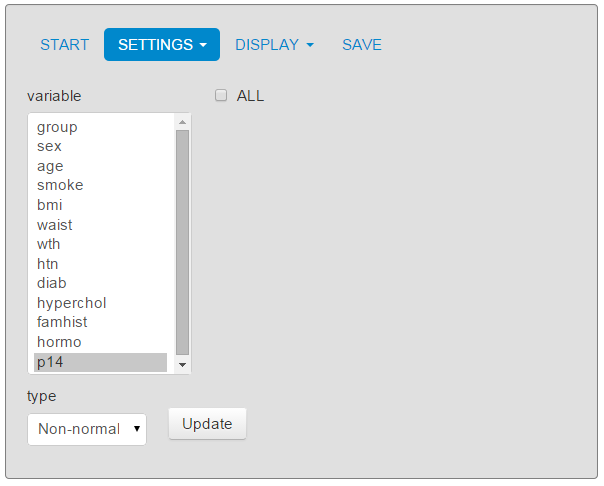
\includegraphics[width=0.55\textwidth]{./figures/WUI/step4a.png}}
\end{center}	

    \vspace{0.5cm}
	\item {\bf Hide:} To hide the `No' category for the (`yes'/`no') variables such as hypertension, diabetes, etc., we will type `No' in the `hide no' input text window. Also, to hide the `female' category for we will select the `sex' variable and `female' category and press `Update' button afterwards.
\begin{center}
\fbox{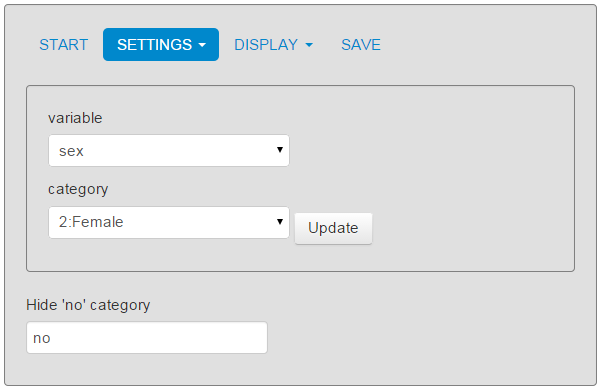
\includegraphics[width=0.65\textwidth]{./figures/WUI/step4b.png}}
\end{center}	

\newpage	
	\item {\bf OR:} Since we have hidden the females, we have to do the same for the HR. Also, for the waist we will change the scale to 5. Doing this, the HR will represent the change in 5 units.
\begin{center}
\fbox{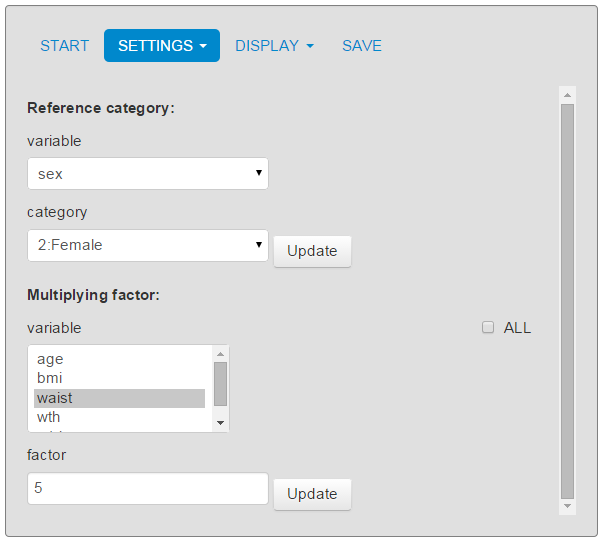
\includegraphics[width=0.65\textwidth]{./figures/WUI/step4c.png}}
\end{center}	

    \vspace{0.5cm}
	\item {\bf Subset:} If we want to do the analysis only for male type `sex==1' or `sex==2' in only females must be analysed in the `global subset' text input window.
\begin{center}
\fbox{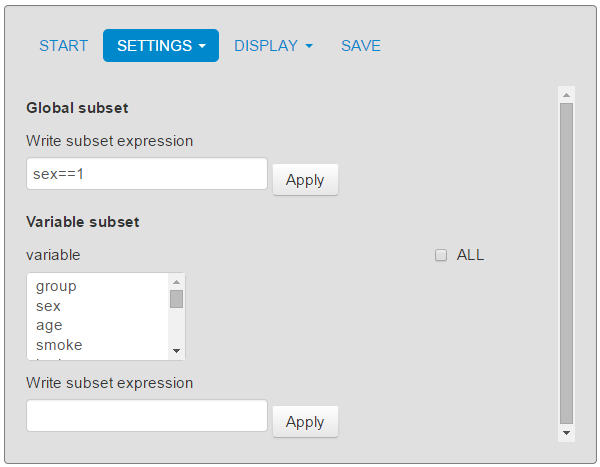
\includegraphics[width=0.65\textwidth]{./figures/WUI/step4d.png}}
\end{center}	

	\end{itemize}
	
\newpage
\item {\bf Step 5. What to be displayed and how.}

	\begin{itemize}

	\item {\bf Show:} Then, we specify which columns (information) to be displayed in the bivariate table. For instance, if we want to display the Odds Ratio, its p-value, but not the descriptives for the entire cohort p.overall:	
\begin{center}
\fbox{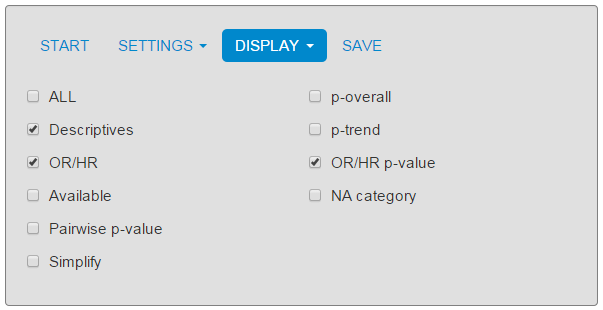
\includegraphics[width=0.65\textwidth]{./figures/WUI/step5a.png}}
\end{center}

    \vspace{0.5cm}
	\item {\bf Format:} Also, we may want to display only the percentages for categorical variables, mean and standard deviation with plus/minus symbol and rounded brackets for first and third quantiles for continuous normal and non-normal variables, respectively:
\begin{center}
\fbox{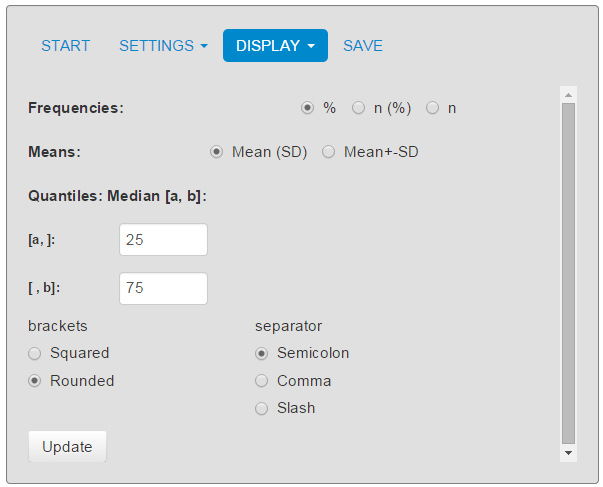
\includegraphics[width=0.65\textwidth]{./figures/WUI/step5b.png}}
\end{center}	

\newpage
	\item {\bf Decimals:} Moreover, it may be important to report more decimals for the odds ratio. By default, two decimals are reported. If we want to report 3 decimals for all variables:
\begin{center}
\fbox{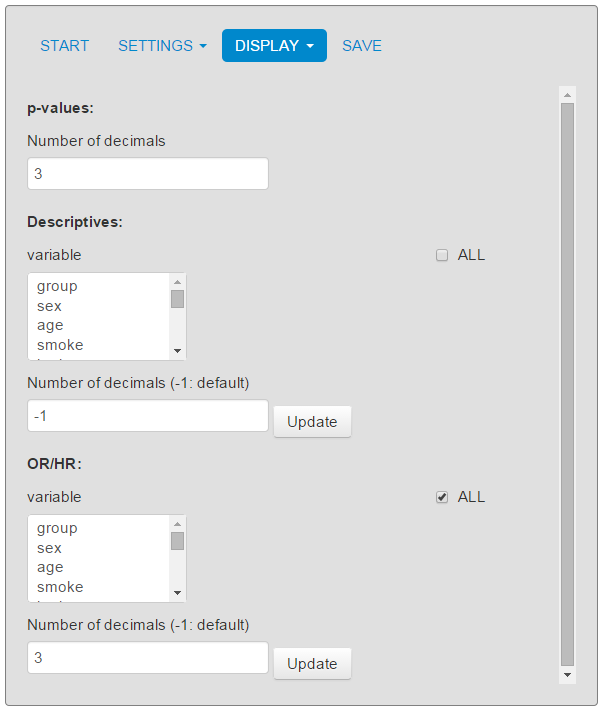
\includegraphics[width=0.65\textwidth]{./figures/WUI/step5c.png}}
\end{center}

	\item {\bf Headers:} Finally, some `key' words in the header of the descriptive tables, (such as `p.ratio', ...) may be changed:
\begin{center}
\fbox{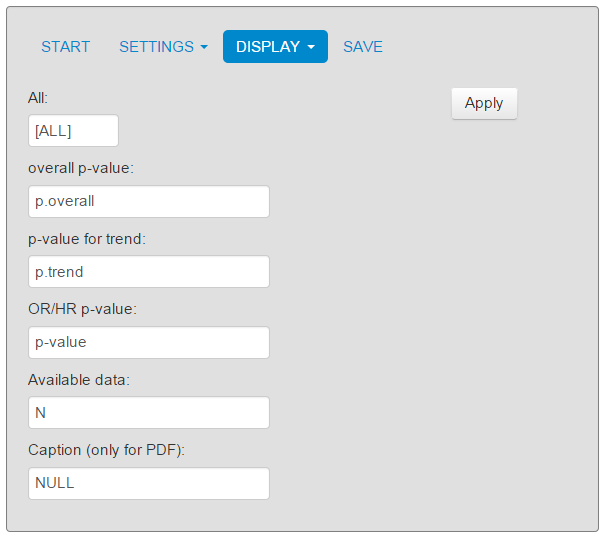
\includegraphics[width=0.65\textwidth]{./figures/WUI/step5d.png}}
\end{center}				

	\end{itemize}

\newpage	
\item {\bf Step 6. Visualize the table:} To see the output, click on TABLE tab on the right panel. The table can be displayed in different formats:

	\begin{enumerate}[i)]
	\item {\bf HTML:}
\begin{center}
\fbox{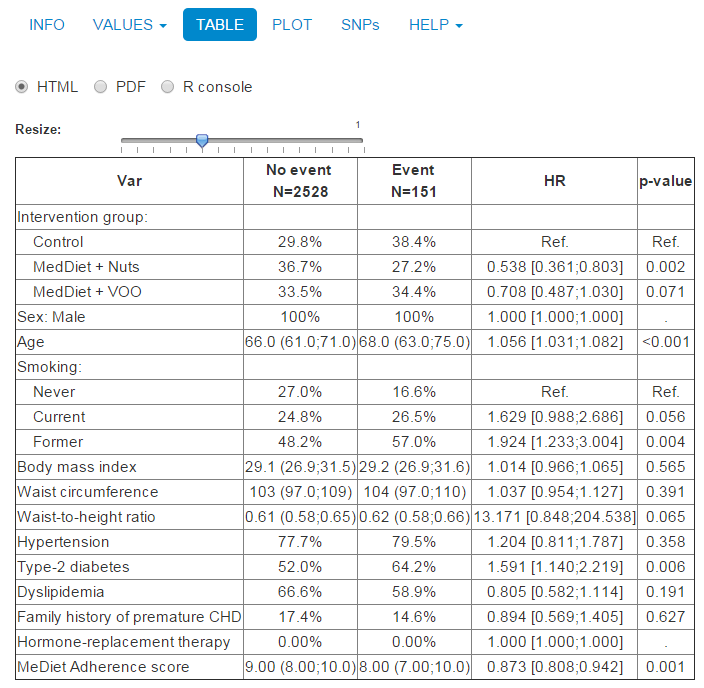
\includegraphics[width=0.65\textwidth]{./figures/WUI/step6a.png}}
\end{center}

    \vspace{0.5cm}
	\item {\bf PDF:}
\begin{center}
\fbox{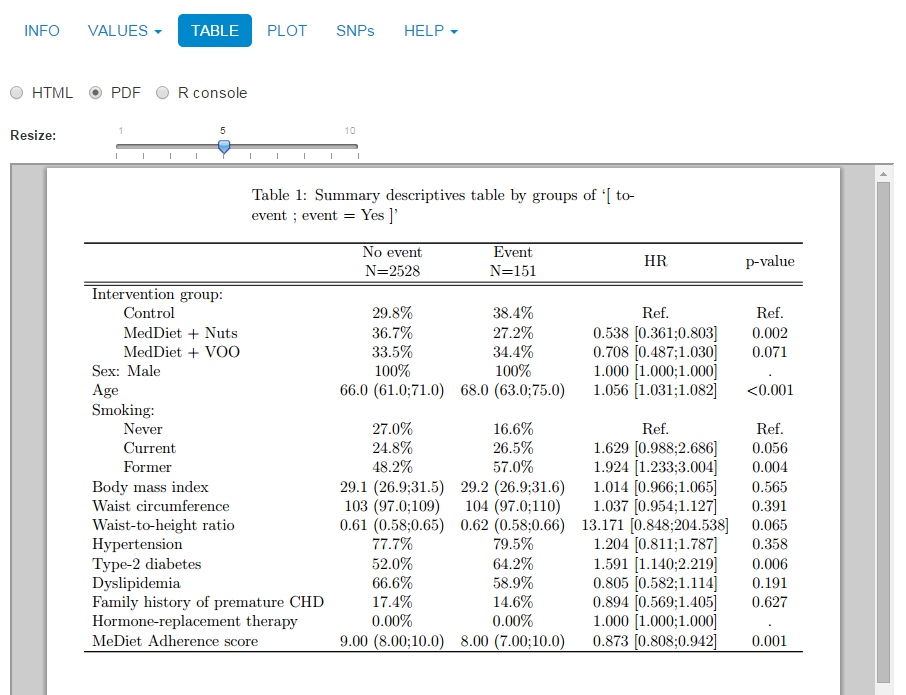
\includegraphics[width=0.65\textwidth]{./figures/WUI/step6b.png}}
\end{center}

\newpage
	\item {\bf {\tt R}:}
\begin{center}
\fbox{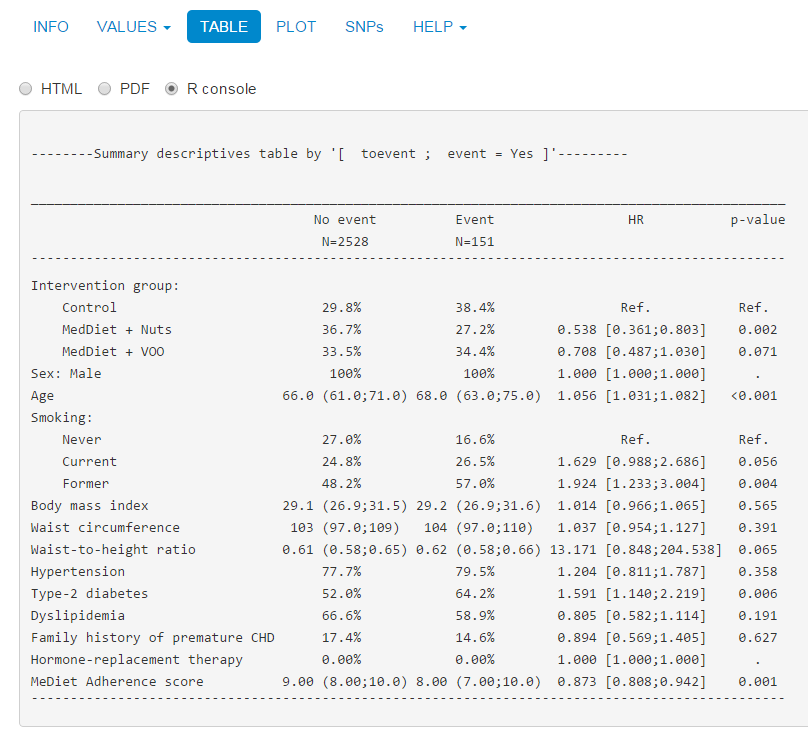
\includegraphics[width=0.65\textwidth]{./figures/WUI/step6c.png}}
\end{center}

	\end{enumerate}

\vspace{1cm}
Note that HTML and PDF formats incorporate an horizontal bar to customize the table size.	

\newpage	
\item {\bf Step 7. Saving the table.} Finally, once the table contains all the desired figures and in the appropriate format, it can be downloaded and stored in different formats:

	\begin{enumerate}[a)]
	\item PDF: a \LaTeX{} compiler such as MikTex must be installed to build the PDF document with the descriptive table. The user can select the font size and whether table must be placed vertically or horizontally (landscape option).
	\item CSV: a plain text file with columns separated by commas or semicolons. For Windows users, this format is useful since it can be opened by Excel.
	\item HTML: a web browser is opened and the table can be easily copied and pasted to  Word, for instance.
	\item TXT: a plain text file which can be opened by any text editor program and which contains the table as in {\tt R} console with a nice format. Once the `download' button is pressed, the file is automatically stored in your PC/Mac.	
	\end{enumerate}
	
\begin{center}
\fbox{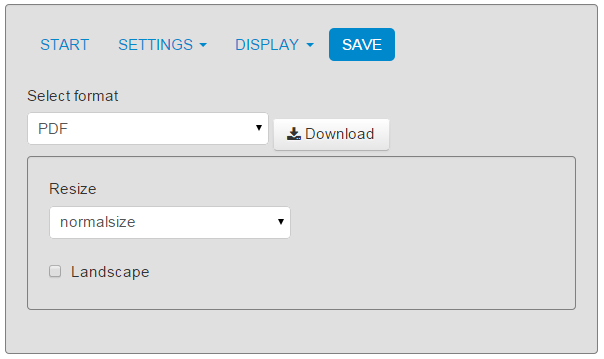
\includegraphics[width=0.55\textwidth]{./figures/WUI/step7.png}}
\end{center}	

	

\end{itemize}


\vspace{2cm}


%\newpage
%\section*{Bibliography}
%\bibliographystyle{bmc_article}  % Style BST file
\bibliographystyle{unsrtnat}  % Style BST file
\bibliography{compareGroups_vignette}

\end{document}

%%%%%%%%%%%%%%%%%%%%%%%%%%%%%%%%%%%%%%%%%%%%%%%%%%%%%%%%%%%%%%%%%%%%%%%%%%%%%
%%%%%%%%%%%%%%%%%%%%%%%%%%%%%%%%%%%%%%%%%%%%%%%%%%%%%%%%%%%%%%%%%%%%%%%%%%%%%
%%%%%%%%%%%%%%%%%%%%%%%%%%%%%%%%%%%%%%%%%%%%%%%%%%%%%%%%%%%%%%%%%%%%%%%%%%%%%
